\documentclass{beamer}
\usetheme{Antibes}
\usecolortheme{dove}
%\usepackage{FiraSans}

\setbeamertemplate{navigation symbols}{}
\setbeamertemplate{itemize items}[default]
\setbeamertemplate{enumerate items}[default]


\usepackage[spanish]{babel}

\title{Atmósfera de Saturno}
\author{Benjamín Ortiz Edwards}
\begin{document}

\frame{\titlepage}

\section{Saturno}

\begin{frame}


\vspace{-2cm}
\begin{figure}
    \centering
    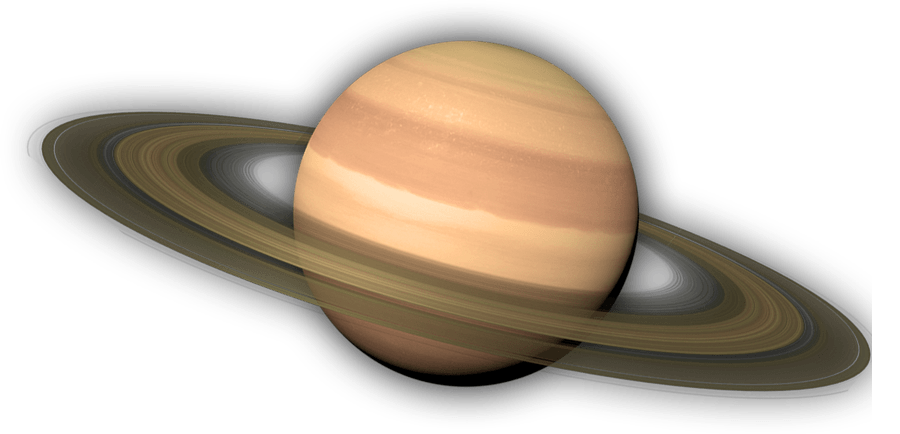
\includegraphics[width=0.6\linewidth]{saturn}
\end{figure}
\begin{itemize}
    \item Saturno es el sexto planeta más cercano al sol y presenta un radio de $\sim 58000$ Km.
    \item El Día y año saturnianos duran 10 horas y 29 años terrestres, respectivamente.
    \item Su apariencia es de colores amarillos y paste, aunque azulado hacia los polos.
    \item Posee bandas ecuatoriales, similares a las de Júpiter.
\end{itemize}
\end{frame}


\section{Composición y estructura}
\begin{frame}{Composición y Estructura}
    \centering
    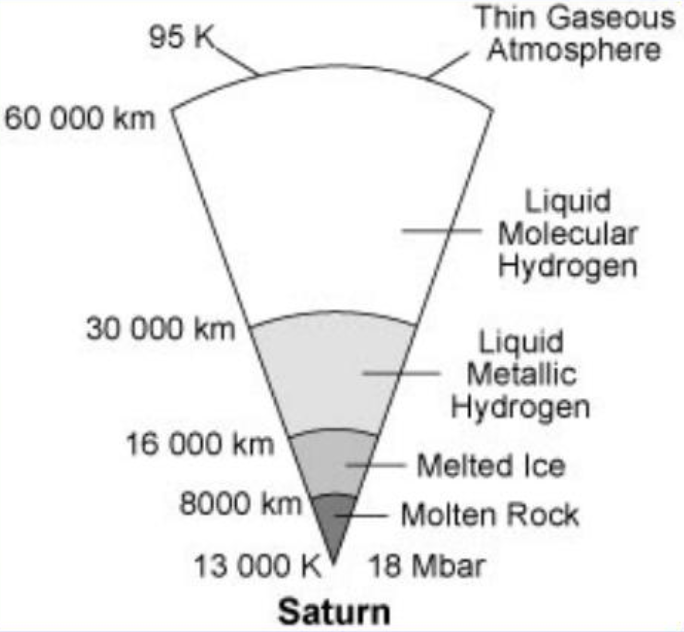
\includegraphics[width=0.4\paperwidth]{saturn_is}
    \begin{itemize}
        \item 96\% de Hidrógeno y 3\% de Helio.
        \item Trazas de	metano, vapor de agua, amoniaco, monoxido de carbono, hidrocarburos, entre otros.	
    \end{itemize}

    \vspace{5mm}

\end{frame}

\begin{frame}
    \begin{minipage}{0.5\linewidth}
    \vfill
    \hspace{-9mm}
    \resizebox{1.1\textwidth}{!}{%
    \begin{tabular}{|l|l|l|l}
        Nubes/Capa & Temperatura & Presión & Composición\\ \hline
        Nubes altas & $\sim$ (100 - 160) K & $\sim$ (0.5 - 2) bar & Amoniaco\\
        Nubes bajas$^1$ & $\sim$ (190 - 235) K & $\sim$ (3 - 6) bar &  NH$_4$SH \\
        Nubes bajas$^2$ & $\sim$ (185 - 279) K & $\sim$ (2.5 - 9) bar & Agua-hielo \\ 
        Capa inferior & $\sim$ (270 - 330) K & $\sim$ (10 - 20) bar & Solución acuosa
    \end{tabular}%
}
\end{minipage}
\hspace{-5mm}
\begin{minipage}{0.4\linewidth}
    \vspace{-1.1cm}
    %\hspace{3cm}
    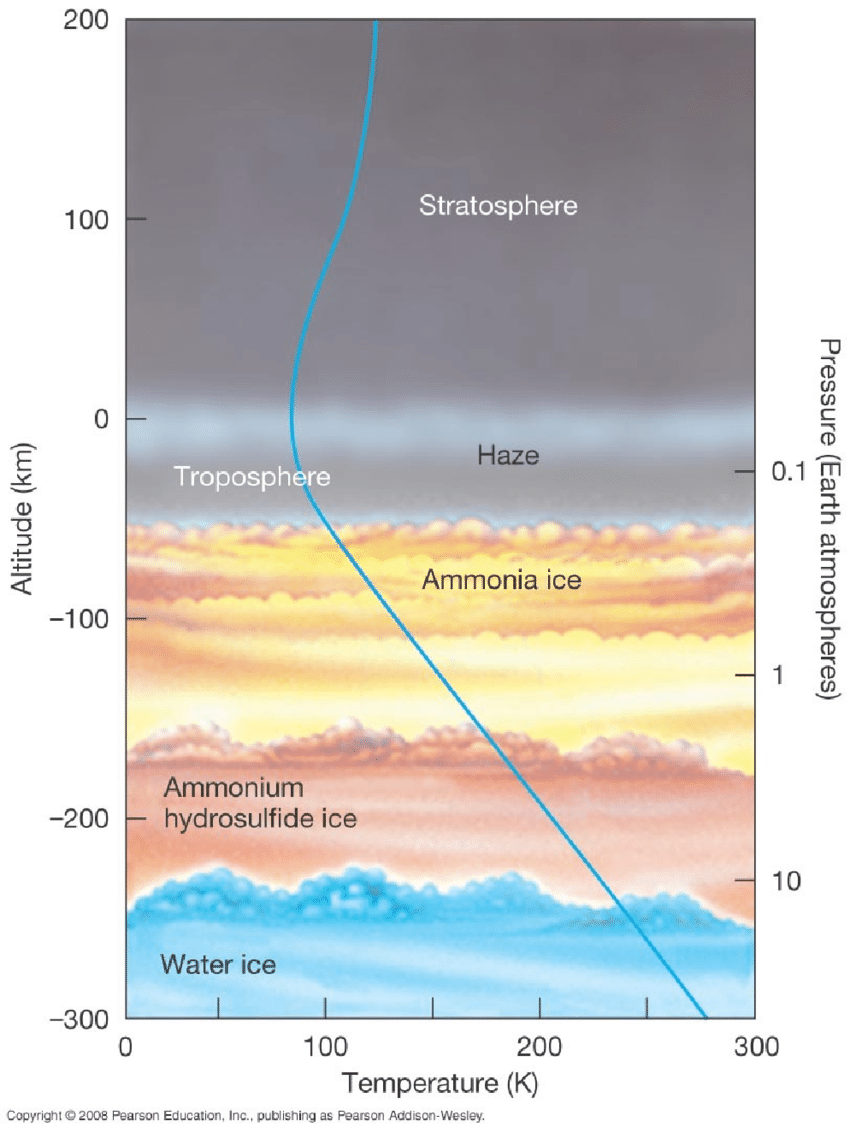
\includegraphics[height=0.90\paperheight]{saturn_atmosphere}
\end{minipage}
\end{frame}


\section{Características}
\begin{frame}{Algunas propiedades}


    \begin{itemize}
        \item Se han detectado vientos en la cima de las nubes que alcanzan velocidades de 1800 Km/h (en el ecuador).
        \item En el mismo polo posee una tormenta con un ``ojo'' bien definido.
            \vspace{3mm}
    \begin{figure}
        \centering
        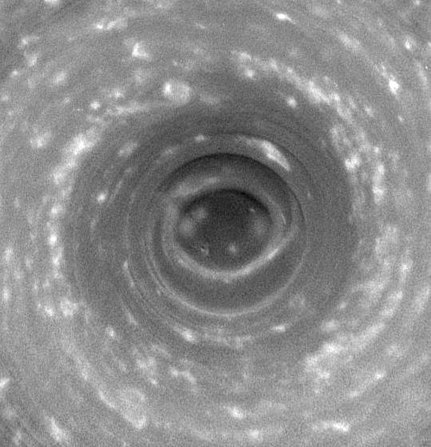
\includegraphics[width=0.35\linewidth]{polar_vortex}
    \end{figure}

    \end{itemize}

\end{frame}


\section{Fenómenos interesantes}
\begin{frame}
    \centering
    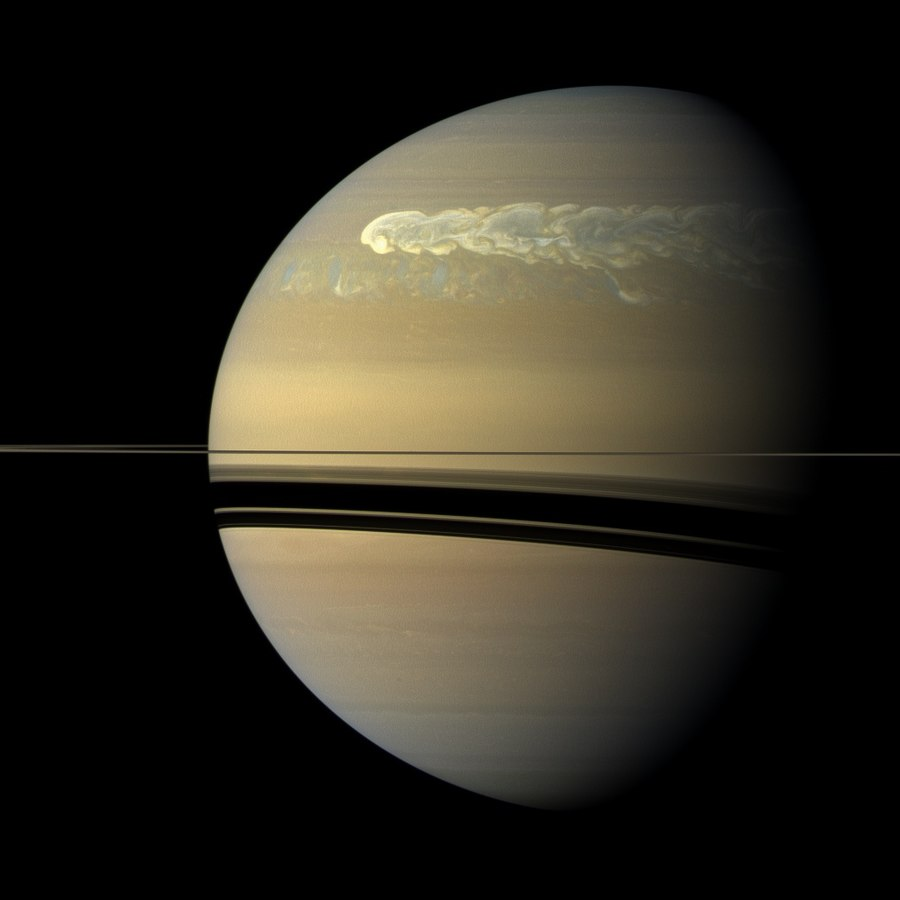
\includegraphics[width=0.7\linewidth]{gws}
\end{frame}

\begin{frame}
    \centering
    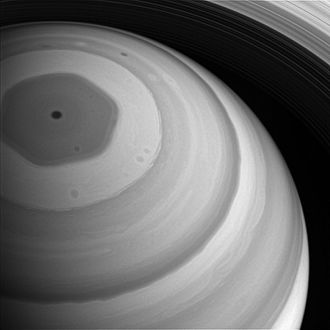
\includegraphics[width=0.7\linewidth]{hexagon}
\end{frame}

\section{Algunas Características}


\section{Referencias}

\begin{frame}{Referencias}
\begin{thebibliography}{9}
    \bibitem{sfc} ``Saturn from Cassini-Huygens'', Dougherty, Michele K. ; Esposito, Larry W. ; Krimigis, Stamatios M. Abstract
    \bibitem{esa} ESA, \url{https://www.esa.int/Science_Exploration/Space_Science/Cassini-Huygens/Saturn_s_atmosphere}
    \bibitem{adp} ``Las atmósferas de los planetas del sistema solar'', Julio Solís García
    \bibitem{image} \url{https://lifeng.lamost.org/courses/astrotoday/CHAISSON/AT312/HTML/AT3120g.HTM}

\end{thebibliography}
\end{frame}
%\frame{\printbibliography}



\end{document}
